\begin{figure*}[t]
	\centering
	\begin{tabular}{cccc}
		\hspace{-0.5em}\subfloat[][$\ammd$ vs. $\mm$ ]{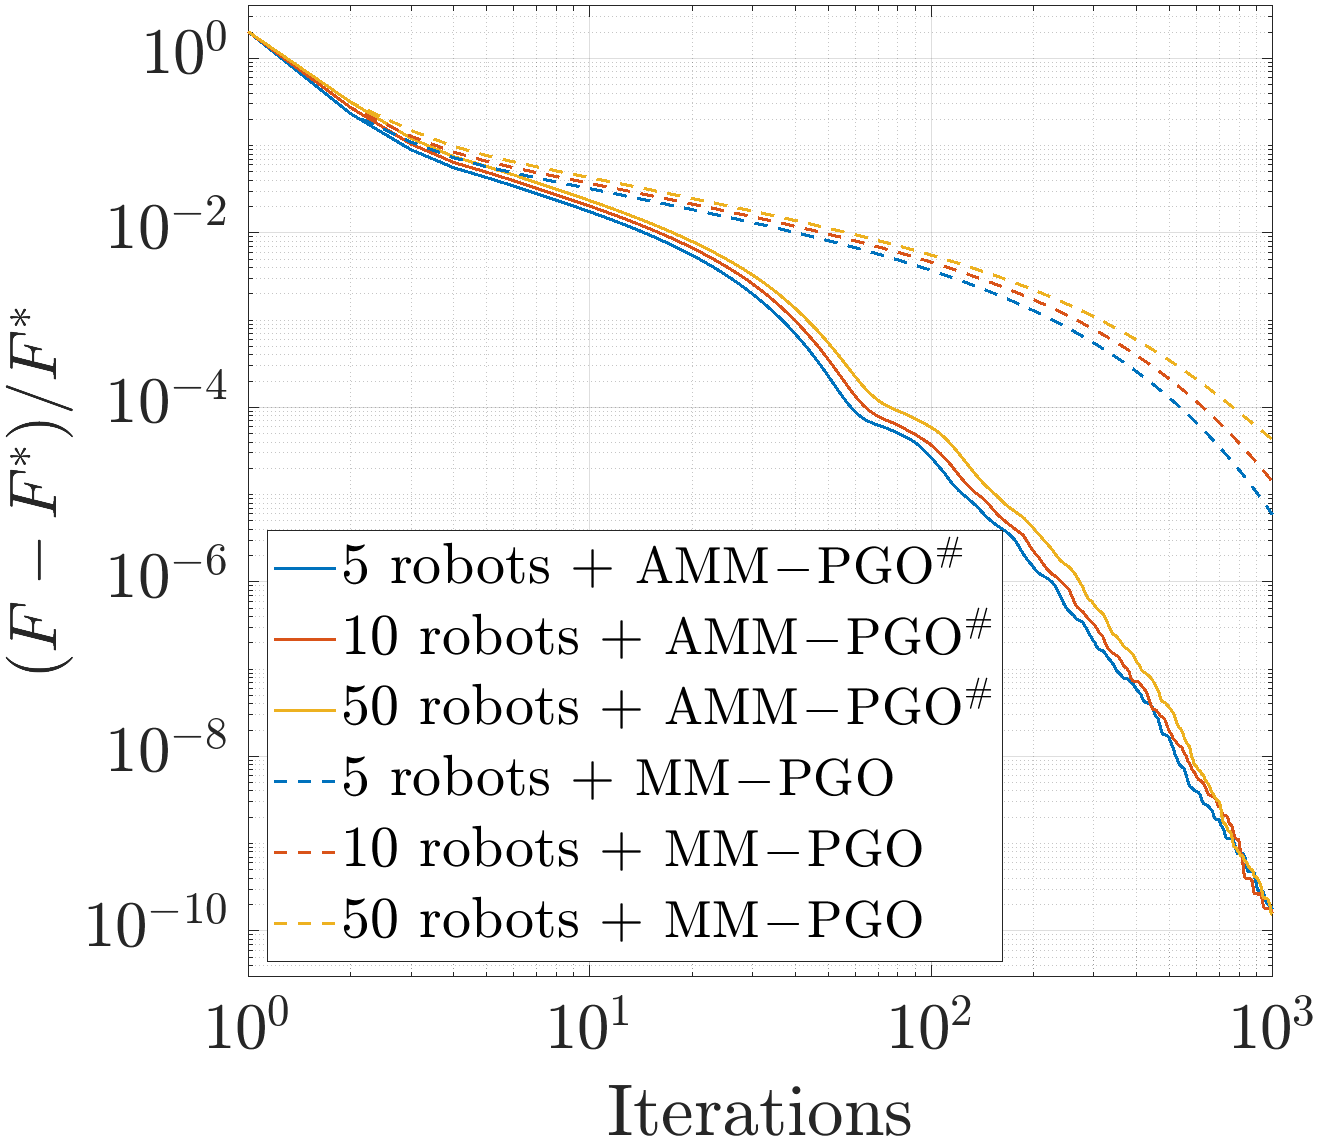
\includegraphics[trim =0mm 0mm 0mm 0mm,width=0.24\textwidth]{figures/cube_tests/rel_none_f.png}} &
		\hspace{-0.6em}\subfloat[][5 robots]{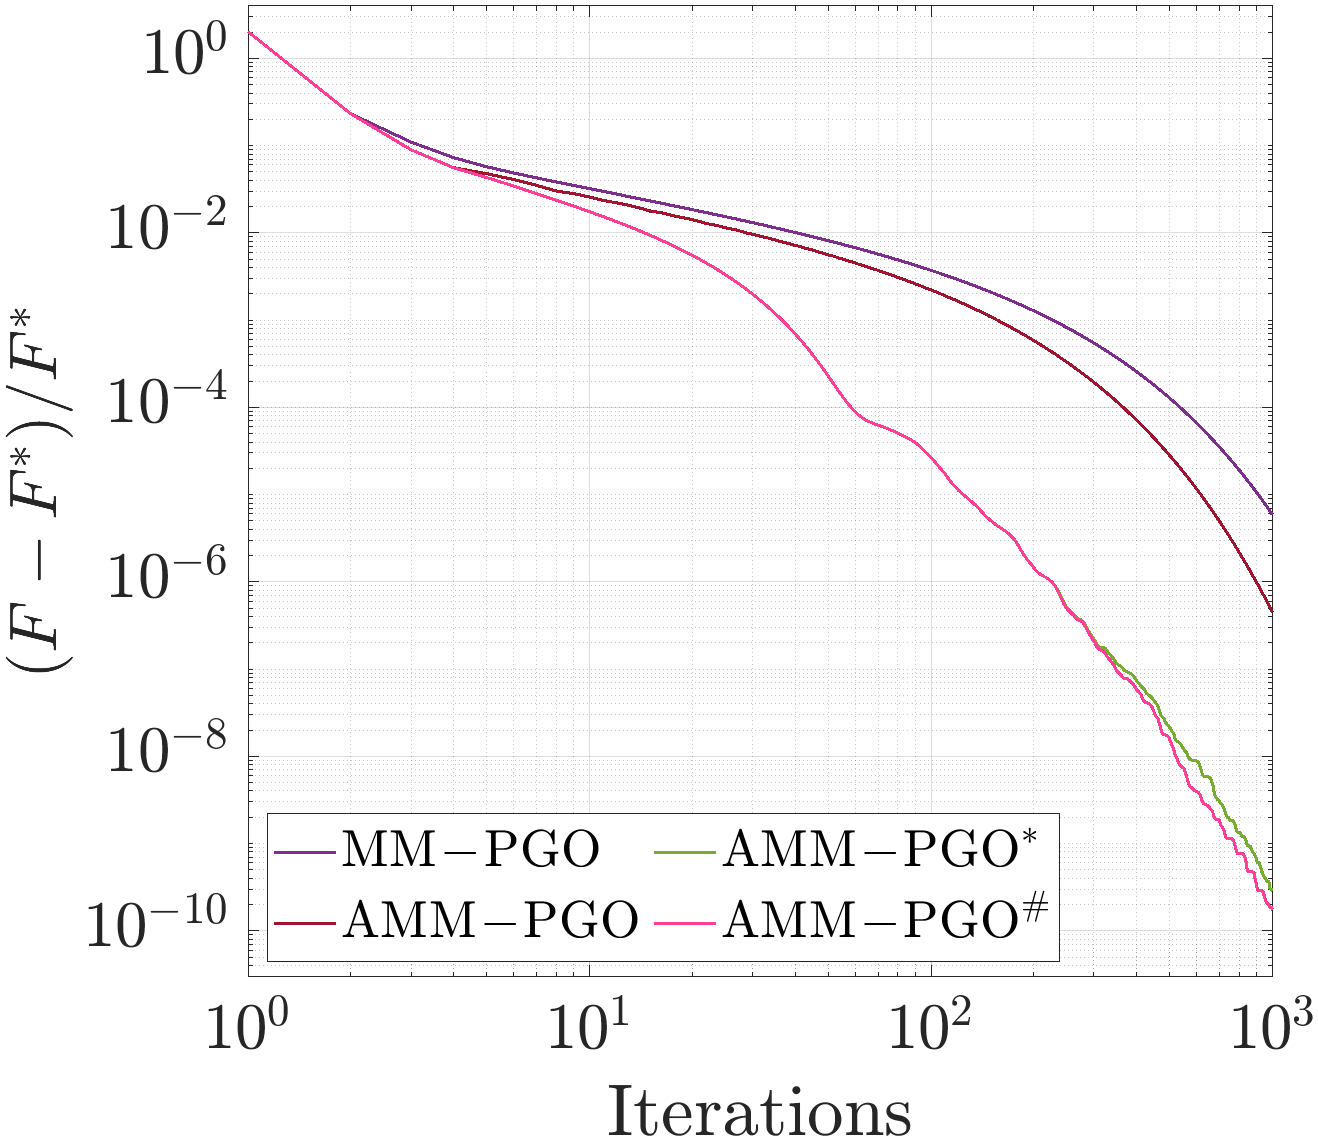
\includegraphics[trim =0mm 0mm 0mm 0mm,width=0.24\textwidth]{figures/cube_tests/rel_none_f_5.png}} &
		\hspace{-0.6em}\subfloat[][10 robots]{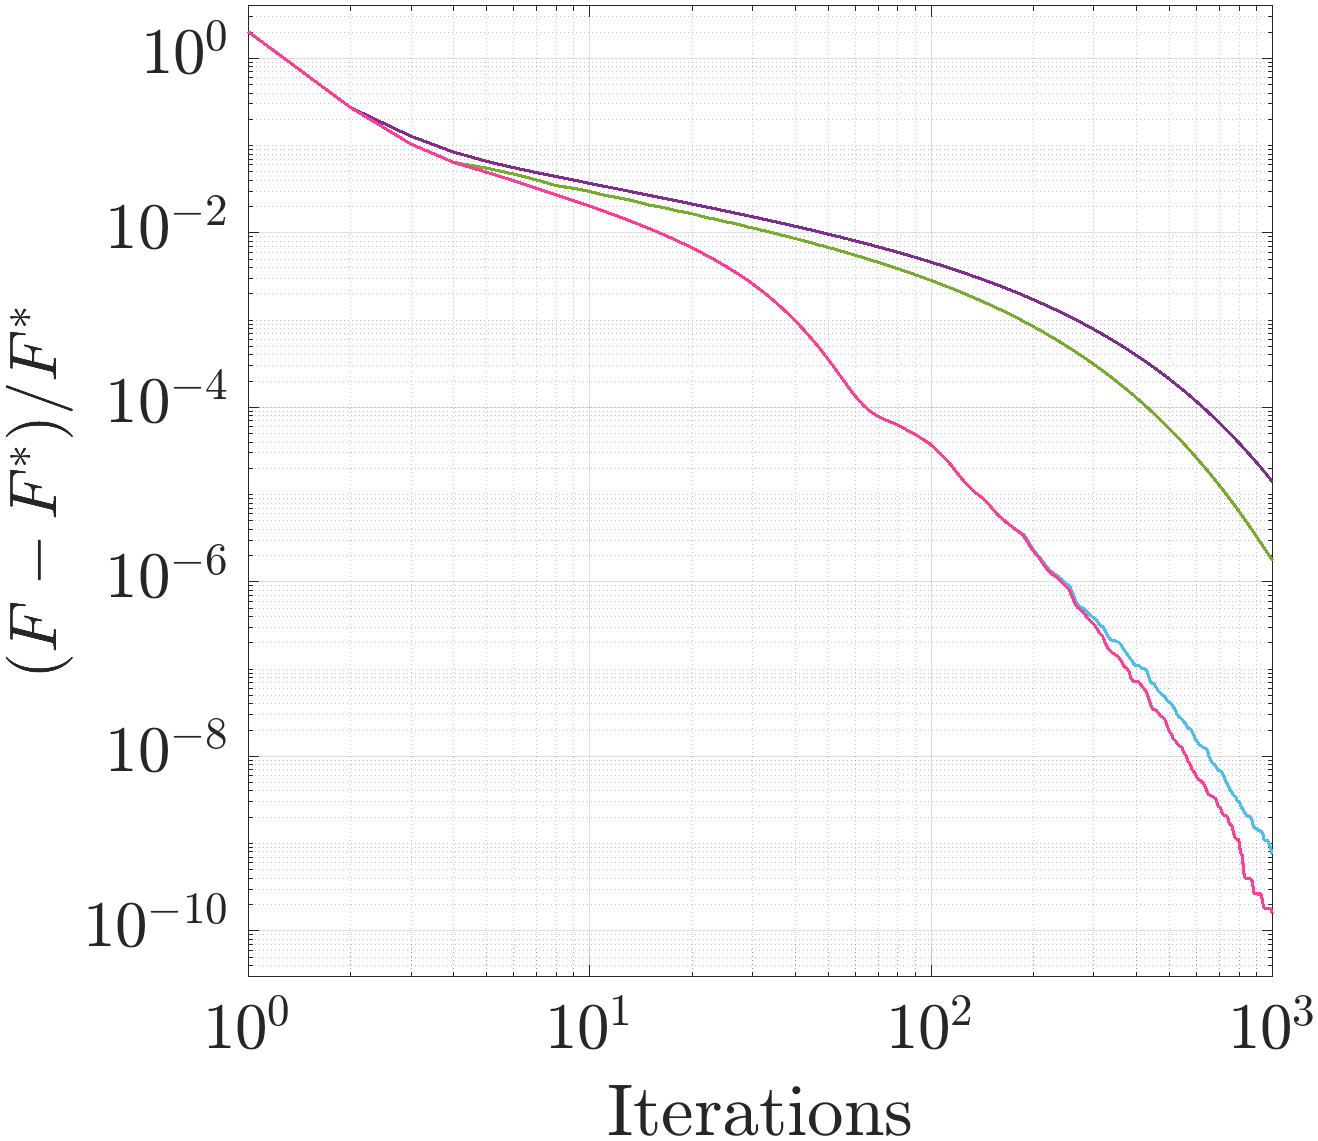
\includegraphics[trim =0mm 0mm 0mm 0mm,width=0.24\textwidth]{figures/cube_tests/rel_none_f_10.png}}&
		\hspace{-0.6em}\subfloat[][50 robots]{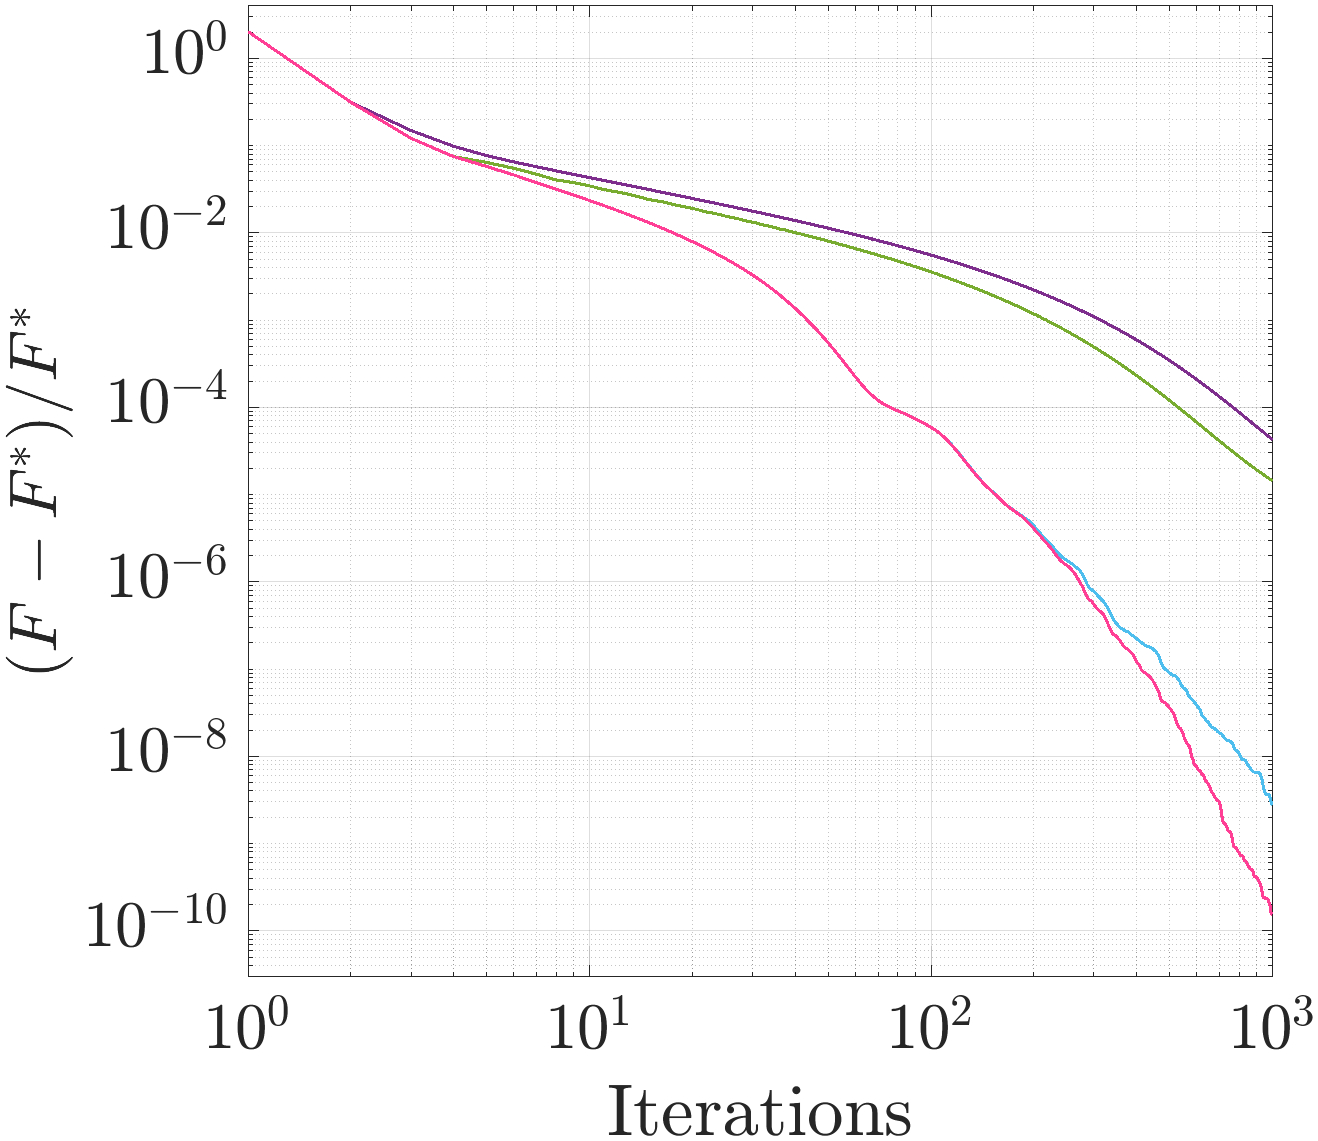
\includegraphics[trim =0mm 0mm 0mm 0mm,width=0.24\textwidth]{figures/cube_tests/rel_none_f_50.png}}
	\end{tabular}
	\caption{The relative suboptimality gaps of the $\mm$, $\ammc$, $\ammd$ and $\amm$ \cite{fan2020mm} methods for distributed PGO with the \textbf{trivial loss kernel} on $5$, $10$ and $50$ robots. The results are averaged over $20$  Monte Carlo runs.}\label{fig::cube_f} 
	\vspace{-1em}
\end{figure*}